\chapter{Theoretical Principles}

\section{Introduction}

Prior to the development of a numerical model it is necessary to give an exact theoretical description of the
fluid systems, which are investigated in the context of this thesis.
Hence this section contains a brief overview of the derivation and the properties of the fundamental equations of motions.
For a more detailed description, the interested reader is referred to \citep{ferziger99} on which section \ref{theorie:eqm1} is based.\\
In the second part of this chapter, the equations will be extended to rotating fluid systems.
The physical solution, known as intertial waves, of this system will be discussed.

\section{The Equations of Motion}\label{theorie:eqm1}

At any time a viscous, newtonian and incompressible fluid is considered. The equations of motion for such a fluid can be derived by considering the conversation of
mass and momentum inside a fixed control volume $V \subset \mathbb{R}^3$.
Within the fluid the momentum at the position $\vec{r} = (x, y, z)^T$  is  characterized by the velocity $\vec{v}(\vec{r}, t) = (v_x, v_y, v_z)^T \in \mathbb{R}^3$,
meanwhile the mass distribution is given by the density distribution $\rho(\vec{r}) \in \mathbb{R}$.

\subsection{Mass Conservation}

Let $\partial V$ be the enclosing surface and $\vec{n}$ the normal vector to the control volume.
We know consider a control mass with the volume $V_M$, traversing the control volume, such that for a fixed point in time it holds that $V_M = V$.
For any intensive property $\phi$ the Reynolds transport theorem states that

\begin{align}
    \label{theorie:reynolds}
    \frac{\dif}{\dif t} \int_{V_M}\dif V \rho \phi  = \frac{\dif}{\dif t}\int_{V} \dif V \rho \phi + \int_{\partial V}\dif S \rho \phi \vec{v} \vec{n}
\end{align}

The assumption of a conservation law requires that the left side of equation \ref{theorie:reynolds} has to be zero.
By setting $\phi = 1$ one obtains the integral form of mass conversation.

\begin{align}
    \frac{\dif}{\dif t} \int_V \dif V \rho(t) + \int_{\partial V}\dif S \rho \vec{v}\vec{n}
     \stackrel{\text{Gauss} \atop \text{ Law}}{=}
    \int_V \dif V \left( \frac{\dif}{\dif t} \rho(t) + \vec{\nabla}\left(\rho \vec{u}\right)\right)
\end{align}

The differential form of the equation is obtained by applying gauss law and considering an infinitesimal small control volume.
\begin{align}
     \frac{\partial \rho}{\partial t}  + \nabla \left(\rho \vec{v}\right) &= 0
\end{align}
As an incompressible fluid is investigated, that is $\rho = \text{const.}$, the incompressible continuity equation reduces to
\begin{align}
     \nabla \cdot \vec{v} &= 0
\end{align}

\subsection{Momentum Conservation}

Using the same approach, but with setting $\phi = \vec{v}$, results in the integral form of the momentum equation

\begin{align}
    \label{theorie:intimpulse}
    \frac{\dif}{\dif t} \int_V \div V \rho \vec{v} + \int_{\partial V} \div S \rho\vec{v}\vec{v}\cdot \vec{n}  =  \sum \vec{F}_{\text{ext.}} + \sum \vec{F}_{\text{int.}}
\end{align}

In addition to the left hand side, the equation is extended by additional internal and external forces, which may act on the fluid inside the control volume.
The external forces depend on the specific physical system, for example the buyont or the coriolis force, whereas the internal forces
are given by the pressure and the normal and shear stresses acting on a fluid element.\\
For a newtonian fluid the internal forces can be described by the stress tensor $\bm{T}$

\begin{align}
    \sum \vec{F}_{int.} = \int_{\partial V}\dif S \bm{T}\vec{n}  = \int_{V} \dif V \nabla \bm{T} =
     \int_{V} \dif V \nabla \left(- \left(p + \frac{2}{3}\mu\nabla\vec{u} \right) + 2\mu \bm{D} \right)
\end{align}
with the static pressure $p$, the dynamic viscosity $\mu$ and the deformation tensor $\bm{D}$.
By applying gauss law to equation \ref{theorie:intimpulse} and consider an infinitesimal volume,
the differential form of the impulse equation, also known as Navier-Stokes equation is than given by
\footnote{The term Navier-Stokes equation is generally referred to as the complete set of equations of motion or
just the impulse equation here we use the latter convention.}
\begin{align}
    \label{theorie:eqns}
    \pdn[v]{t} + \underbrace{\left(\vec{v} \vec{\nabla}\right) \vec{v}}_{\text{I}} &= \underbrace{- \frac{1}{\rho} \nabla p + \nu \Delta \vec{v}}_{\text{II}} +\sum \vec{F}_{\text{ext.}}
\end{align}
where  the kinematic viscosity is given by the definition $\nu = \mu/\rho$.
For an incompressible fluid the force term generated by $\bm{T}$ reduces to (II).\\
Altogether the internal force is now given by the pressure gradient and an diffusive impulse transport proportional to $\nu$.
The non-linearity of the fluid originates through term (I), which is also denoted as the advection operator.
It basically describes the change of impulse of a fluid element when moving through the velocity field.
\footnote{For example the velocity of a fluid element will change when no forces but a velocity field is present.}
It should be noted that the set of equations is not yet solvable as the pressure variable is still undetermined.

\subsection{Initial State and Boundary Conditions}

The solution of a partial differential equation, if it exists, is always undetermined by a constant of integration.
In order to determine the temporal evolution of a fluid system, it is necessary to define its initial state and therefore
to determine one specific solution.\\
This means that for every variable we have to choose an initial condition.
With respect to a numerical solution it has to be considered that, for example an instability, is always triggered by some kind of disturbance.
Thus it might be advisable to not choose a trivial solution like a zero velocity field, but instead a solution which quickly evolves in the state
of the system one wants to achieve. Many times it is useful to add pseudorandom noise.\\
\\
Since the fluid domain is spatial restricted it is as well necessary to define the physical behavior at its boundaries.
For a fluid domain $V$ with the boundary $\partial V$, the following boundarys are considered, as defined in \citep{Griebel1998} and \citep{ferziger99}.

\begin{description}
    \item[No-Slip Boundaries] All velocities components are set to zero $\vec{v}|_{\partial V} = 0$. The fluid is at rest on $\partial V$ and no flux through
                              the boundary occurs.
                              In a more general case, this kind of condition is  also referred to as Dirichlet-Condition where $\Phi|_{\partial V} = c\in\mathbb{R} $,
                              for any variable $\Phi$.

    \item[Free-Slip Boundaries] The velocity component in normal direction to the wall is set to zero, hence $\vec{n} \nabla \vec{v} = 0$ and $\vec{n}\vec{v}=0$ is required.
                                No flux through $\partial V$ occurs and no friction is imposed on the fluid.

    \item[No-Flux Boundaries] For a scalar $\Phi$, the flux through the boundary is zero, hence $\vec{n}\nabla \Phi = 0$.
                              Here the general case is referred to as Neumann boundary condition, where $\vec{n}\nabla \Phi = c\in \mathbb{R}$.
                              This boundary conditions is used i.e. to avoid energy flux through the domain boundary.

    \item[Periodic boundaries] Periodic boundaries can be applied in all directions of a system. For example if the system is periodic in x-Direction with a period of length $L$,
                                one has to ensure that all variables match on the boundaries, that is $\Phi(x) = \Phi(x + L)$, for any variable $\Phi$.
\end{description}

\subsection{Nondimensionalization}

For many fluid systems nondimensionalization is used to further simplify the equations of motion and reduce the number of free parameters.
The approach behind this scheme is to define variable substitutions, such that the overall systems is free from any physical units.\\
After the nondimensionalization the system is described by one or more dimensionless quantity, which characterize the overall physical behavior.
As a result it is easier to compare numerical simulations and experimental setups to one another.
We can choose the following scales for the variables of time, position, velocity and pressure (see \cite{Kundu2012}), the nondimensional variables are denoted by an asterisk.

\begin{align}
    \text{Length:}\qquad &  \vec{r}^* = \frac{\vec{r}}{L}  & \qquad \text{Velocity:}\qquad& \vec{v}^* = \frac{\vec{v}}{V}\\
    \text{Time:}  \qquad & t^* = t \cdot \frac{V}{L}      & \qquad  \text{Pressure:}\qquad & p^* = \frac{p - p_\infty}{\rho V^2}
\end{align}

where  $L$ is a length and $V$  a velocity, given by characteristic scales from the fluid system, which is examined.
The pressure scale is set as a difference with respect to a characteristic pressure $p_\infty$.
With the above defined scales the nondimensionalized Navier-Stokes equation is given by \footnote{
From now on we ignore the * for all dimensionless variables }:

\begin{align}
    \pdn[v]{t} + \vec{v} \cdot \vec{\nabla} \vec{v} &= -\nabla p + \frac{1}{Re} \Delta \vec{v} + \vec{F}_{ext.}
\end{align}

The dynamic of the system is reduced to the dimensionless quantity $\Rey$, also referred to as the Reynolds number,
defined by (\citep{Kundu2012}):

\begin{align}
    \label{theorie:renumber}
    Re := \frac{VL}{\nu} = \frac{\rho VL}{\mu}
\end{align}

\newpage

From equation \ref{theorie:renumber}, it can be seen that the Reynolds number gives the ratio between the inertial forces $\propto VL$
to the viscous forces $\propto \nu$, of the fluid system.
This means that for a small Reynolds numbers the viscosity determines the flow, a laminar flow can be expected.
For a large Reynolds number an  advection driven, maybe even turbulent flow, dominates.\\

%To illustrate the behaviour, figure \ref{theorie:re_example} exemplarly shows the airflow around a cylinder at different reynolds numbers.
%TODO:\\
%- bild\\
%- comparison\\
%
%\begin{figure}[!pb]
%    \label{theorie:re_example}
%  \centering
%    \missingfigure[figwidth=\textwidth]{Flow over a cylinder for different Reynolds numbers}
%\end{figure}
%\newpage
\clearpage

\section{Rotational Fluid Dynamics}

In this section the Navier-Stokes equations are extended to govern the physical attributes of rotating systems,
which play an important role in the context of geophysical fluid dynamics.\\
Due to the continuous acceleration acting on the fluid, these systems exhibit some fundamental different behavior, than one would expect.
One important case which shall be discussed, is the propagation of inertial waves inside a stratified rotating fluid.\\

\subsection{Equations of Motion}
\label{THEORIE:ROT}

We initially consider the motion of fluid in a coordinate system (\textbf{R}), rotating relative to the intertial system (\textbf{I}) around the axis $\vec{\Omega}$.
The relation of the time derivate between the two frames of motion is given by the relation
\begin{align}
    \left.{\pdn[]{t}}\right|_{\bm{I}} = \left.\pdn[]{t}\right|_{\bm{R}} + \Omega \times
\end{align}
according to \citep{Tilgner2007}.
Applying this relation to the position vector relative to the coordinate systems \textbf{R} and \textbf{I}
and by furthermore assuming a constant rotation rate, thus $\partial_t\vec{\Omega} = 0$, yields a coordinate transformation for the acceleration.

\begin{align}
    \label{theorie:rottrafo}
    \left.\pdn[\vec{v}]{t}\right|_{\bm{I}} = \left(\left.\pdn[\vec{v}]{t}  + \underbrace{2\vec{\Omega} \times \vec{v}|_R}_{\text{I}}
    - \underbrace{\vec{\Omega} \times (\vec{\Omega} \times \vec{r|_R}}_{\text{II}})\right)\right|_{\bm{R}}
\end{align}

Hence, the transition into a rotating coordinate system introduces two additional translucent forces, the coriolis force (I)  and the centrifugal force (II).\\
A substitution of expression \ref{theorie:rottrafo} into the Navier-Stokes equation gives the equations of motion for the rotating system.
A further simplification can be obtained by considering that the centrifugal force is independent of the velocity field,
hence it can be written in terms of a potential $\Phi$

\begin{align}
    \Omega \times (\Omega \times \vec{r}) = - \nabla \left(\frac{1}{2}\Omega^2\vec{r}^{'2}\right) = -\Phi
\end{align}

which can be substituted into the pressure gradient by defining $p^* = p - \Phi$ \citep{tritton88}.
\newpage
Last but not least the following scales are introduced to obtain a nondimensional equation

\begin{align}
    \text{Length:}\qquad &  \vec{r}^* = \frac{\vec{r}}{L}  &
    \qquad \text{Velocity:}\qquad& \vec{u}^* =  \frac{\vec{u}}{|\vec{\Omega}|L}\\
    \text{Time:}  \qquad & t^* = t \cdot |\vec{\Omega}| &
    \qquad  \text{Pressure:}\qquad & p^* = \frac{p - p_\infty}{\rho L^2{|\vec{\Omega}|}^2}
\end{align}

The final nondimensionalized form of the Navier-Stokes equation for the rotating coordinate system reads

\begin{align}
    \label{theorie:rotns}
    \pdn[v]{t}+ \left(\vec{v}  \vec{\nabla}\right) \vec{v} + 2\Omega \times \vec{v}  &= -  \nabla p + \Ekman \Delta \vec{v} + \vec{F}_{\text{ext.}}
\end{align}

with the dimensionless quantity $\Ekman$ the Ekman-Number, which is defined by

\begin{align}
    \Ekman := \frac{\nu}{|\vec{\Omega}| L^2} \hat{=} \frac{\text{viscous forces}}{\text{coriolis forces}}
\end{align}

The Ekman number describes the ratio between viscous and coriolis forces.

\subsection{Inertial Waves}

One solution of Eq. \ref{theorie:rotns} are inertial waves, which will be described here.
We begin this section by briefly recapture some of the fundamental properties of mechanical waves, as quoted by \cite[p.194]{Kundu2012}.

\begin{quote}
It is perhaps not an overstatement to say that wave motion is the most basic feature
of all physical phenomena. Waves are the means by which information is transmitted
between two points in space and time, without movement of the medium across the
two points. The energy and phase of some disturbance travel during a wave motion,
but motion of the matter is generally small. Waves are generated due to the existence of
some kind of “restoring force” that tends to bring the system back to its undisturbed
state, and of some kind of “inertia” that causes the system to overshoot after the
system has returned to the undisturbed state.
\end{quote}

The propagation of inertial waves requires a medium which contains a state of equilibrium and
a restoring force pointing back to this state in response to a disturbance.
In the context of geophysical fluid mechanics an equilibrium state can be given by a stratification.\\
Consider for example a fluid with a continuous stratified density.
This means that in the equilibrium, the density of the fluid has to decrease
continuous with the height of the system. The displacement of a fluid element
 from its resting position results in a restoring force, which is  given by the
gravitation or the buoyant force.
\footnote{This depends on the direction of the displacement}
It can be seen therefore, that a disturbance of the equilibrium state can result in the
propagation of so-called  gravity waves \cite{Clausen2011}.
\footnote{One import case we know from everyday life are surface waves, which emerge
from the discontinuous density stratification between two fluids, i.e. water and air \cite{Clausen2011}.}\\
We know consider a uniform rotating fluid without the presence of external forces.
At some point in time a steady state is reached, as a result of the dynamic equilibrium between
a radial stratification of the angular momentum and the pressure.
The displacement of a fluid element in radial direction now results in
an imbalance of the preserved angular momentum and the pressure.
Due to the restoring force, given by the coriolis force, an oscillation develops.
Waves of this type are denoted as inertial waves \cite{Clausen2011}.

\subsubsection{Plane Inertial Waves}

Here a short introduction of the porperties of plane inertial waves shall be given.
All results presented in this section are adopted from \citep{Greenspan1990}.%[p.185]
The non-linear advection operator and the viscous stress in Eq. \ref{theorie:rotns} are neglected, $\Ekman =0$.
In case of the a linear inviscid fluid, the equations of motion are fullfiled by plane wave solutions of the form

\begin{align}
    \vec{v} = \vec{V} e^{i(\vec{k}\vec{r}  - \omega t )}, \qquad
    p = P e^{i(\vec{k}\vec{r}  - \omega t )}
\end{align}

The wave is transverse, since an insertion into the continuity equation yields $\vec{V}\vec{k} = 0$.
From the momentum equation the dispersion relation is given by

\begin{align}
    \label{theorie:eq_rot_dispersion}
    \omega = \pm \frac{ 2\vec{\Omega}\vec{K}}{|\vec{K}|} = \pm 2|\vec{\Omega}|\cos(\theta)
\end{align}

where $\theta$ is the polar angle with respect to the rotation axis,
such that $\vec{K}\vec{\Omega} = |\vec{K}||\vec{\Omega}|\cos{\theta}$.
This means that an inertial wave can only exist for a wave frequency smaller than twice of the rotation rate $\vec{\Omega}$.
The phase velocity $\vec{c}_p$ and the group velocity $\vec{c}_g$ are given by

\begin{align}
    \vec{c}_p = 2 \frac{\vec{\Omega} \vec{K} }{|\vec{K}|^3} \vec{K}, \qquad
    \vec{c}_g = \frac{2 \vec{K} \times (\vec{\Omega} \times \vec{K})}{|\vec{K}|^3}
\end{align}

\clearpage


It can be noted that the group velocity and therefore the energy transport is perpendicular to the phase velocity of the wave.
The direction of propagation on an inertial wave is given by the angle $\theta$ with respect to the axis of rotation $\vec{\Omega}$,
see Fig. \ref{theorie:reflection_img}(a).


\subsubsection{Reflection of Inertial Waves}
\label{theorie:sec:iwreflec}

The reflection of an inertial wave contradict's snells law, since the propagation angle $\theta$ is preserved upon a reflection.
It can be shown that the following relations holds (see \cite{Beardsley1970}),

\begin{align}
\label{theorie:reflections}
\vec{\Omega}\cdot \vec{K} =  \vec{\Omega}\cdot\vec{K}^\dagger, \qquad \hat{n} \times \vec{K} = \hat{n} \times \vec{K}^\dagger
\end{align}

where $\dagger$ denotes wave number upon reflection and $\hat{n}$ corresponds to the the normal vector of the wall.
As a result inertial waves exhibit a fundamental different reflection behavior, which shall be summarized here.
Fig. \ref{theorie:reflection_img} exemplarily shows the reflection of an inertial wave with propagation angle $\theta$,
on a wall with the slope $\alpha$ to the rotation axis. Three scenarios exist \citep{Clausen2011}:

\begin{description}
    \item[$\theta < \alpha$] See Fig. \ref{theorie:reflection_img}(b). A downward propagating wave is reflecting upwards,
                             this is also referred to as subcritical reflection.
                             The distance between to parallel waves is decreased upon a reflection which is denoted as focusing.
    \item[$\theta > \alpha$] See Fig. \ref{theorie:reflection_img}(c). A downward propagating wave is reflecting downwards.
                             this is also referred to as supercritical reflection.
                             The distance between to parallel waves is decreased upon a reflection which is denoted as defocusing.
    \item[$\theta = \alpha$] All waves are reflected parallel to the slope and infinitely focussed.
\end{description}

\begin{figure}[!bp]
      \centering
        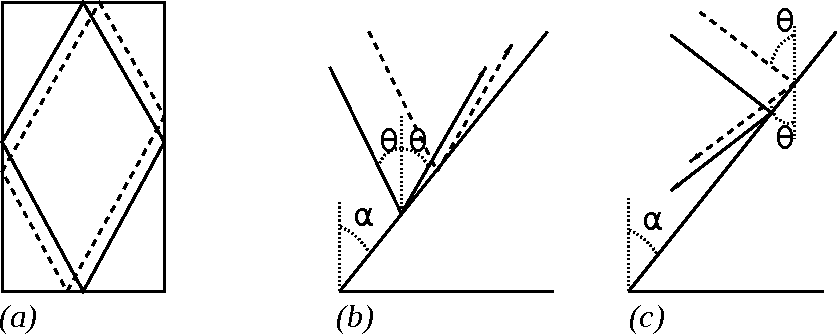
\includegraphics[width=0.7\textwidth]{gfx/theorie/reflection.pdf}
       \caption{Reflection of inertial waves, apapted from \citep{Clausen2011}.
        (a) Propagation of inertial waves with the propagation angle $\theta$.
        (b) Subcritical reflection of a downward traveling wave.
        (c) Supercritical reflection of a downward traveling wave.
       }
       \label{theorie:reflection_img}
\end{figure}

\clearpage


\subsubsection{Inertial Modes in a Cylinder}
\label{theorie:rotating:cyl_modes}

In a closed geometry the possible number of solutions of Eq. \ref{theorie:rotns} can be finite \citep{Clausen2011}.
For the scenario of a rotating cylinder the solutions are given by a discrete spectrum of  inertial modes.
A theoretical solution can be found in \citep{Greenspan1990}, and shall be summarized here.

For the linear inviscid case with $\Ekman~=~0$ and without the advection term, the problem can be reduced to a Poincar\'{e} equation for the pressure,
which is solved in cylindrical coordinates by

\begin{align}
    p_{nmk}(r, \theta, z, t) = J_{|k|}\left(\frac{\xi_{nmk}r}{a} \right)\cos(n\pi)e^{ik\theta}e^{i\lambda t}
\end{align}

where $a=\nicefrac{r}{H}$ is the aspect ration of the cylinder,
$n\in\mathbb{N}$ is the vertical and $k\in\mathbb{Z}$ the azimuthal wave number.
$m\in\mathbb{N}$ is equal to the number of nodes in radial direcion.
$J_{|k|}$ denotes a Bessel function of $k$-th order.
The radial wavenumber $\xi$  can be solved for any given $k$ by the transcendental equation
\begin{align}
    \xi \frac{\dif}{\dif \xi}J_{|k|}(\xi) + k \sqrt{1 + \frac{\xi^2}{n^2\pi^2a^2}} \; J_{|k|}\left(\xi\right) = 0
\end{align}
Finally the eigenvalue of the solution is determined by
\begin{align}
    \lambda_{nmk} = 2\sqrt{1 \; + \;\frac{ \xi_{nmk}^2}{n^2\pi^2a^2}}
\end{align}

%
%\subsection{Ekman schicht}
%
%\subsection{Properties of the Ekman number}
%liste mit eigentschaften
%breite ekmanschicht breite
%spinup
%dämpungsrate welle evtl
%



